\documentclass{article}
\usepackage[utf8]{inputenc}
\usepackage[margin=1in]{geometry}
\usepackage{hyperref}
\usepackage{graphicx}
\usepackage{subfiles}
\usepackage{makecell}
\usepackage{float}

\title{PredictChain}
\author{Matthew Pisano, Connor Patterson, William Hawkins}
\date{Spring 2023}

\begin{document}

    \maketitle

    \section{Project Description}

    PredictChain is a marketplace for predictive AI models. Users are able to upload datasets for training predictive models,
    request that some basic models be trained on any previously uploaded datasets, or submit queries to those trained models.
    These various models will be operated by a central node or nodes with computing resources available. A variety of
    models will be made available, ranging from cheap, fast, and simple to more expensive, slower, and more powerful.
    This will allow for a large variety of predictive abilities for both simple and complex patterns.  All the past
    predictions form these models will be stored on the blockchain for public viewing.

    \subsection{Problem Solved}
    % Clearly state the problem your project solves

    PredictChain helps to solve one of the main issues that involve AI models today: accessibility.  Our project fulfils this
    need in two ways.  Oftentimes, individuals or groups poses data that they would wish to be used in predictive analysis.
    However, these people may not have access to the compute capacity to train predictive models on this data.  Additionally,
    yet other people have neither access to predictive training data, nor do they have access to computational resources.
    PredictChain solved both of these problems simultaneously.

    When users upload their datasets, they allow model to be trained on those datasets.  Higher quality datasets will produce
    higher quality models.  When users submit parameters for training, they allow the model that their parameters produce to
    be used publicly.  Both of these users are rewarded for their work when a model is queried, and it produces a correct
    prediction.  This encourages users to participate in contributing the resources needed for good predictions, while
    leaving a public record for other users to view.

    \subsection{Background}
    % Why is this an important and relevant problem within the context of AI and Blockchain

    As the trend of ever-growing machine learning models continues, this problem becomes increasingly relevant.
    As the scale and power of these models grow, the resources required to train them grow as well.  This makes training
    useful machine learning models unattainable for most people.  In order to get useful results from these models,
    users often have to pay large, centralized organizations, without any reward if they provide a good dataset or model
    parameters.  PredictChain changes this paradigm by incentiveizing the thoughtful creation of useful models and
    datasets.

    Additionally, after the recent mania and subsequent crash around blockchain adjacent technologies, it has become
    important to remind people that blockchains can be used for genuine utility in addition to investment.  By primarily
    using Algos as a method of payment, instead of investment, it helps to, once again, show that cryptocurrencies can
    effectively be used as a pure form of payment for useful services.  Of course, this is in addition to the many other
    services that use crypto in a similar manner, but adding one more project only helps the Algorand's notion of usefulness.


    \subsection{Use Cases and User Stories}
    % Use case or motivating user story detailing how someone would use the system you have built

    \subsubsection*{User Story \#1}
    \textit{Scenario:} As a data analyst, I want to have access to trends of various stock markets so that I can create
    predictive models that will inform my investment strategies.

    \subsubsection*{User Story \#2}
    \textit{Scenario:} As a stockbroker, I want to compare my dataset to another dataset against the same model so that
    I can get an idea as to which is better.

    \subsubsection*{Use Cases}
    For the sake of space, we will only go over two simple Use Cases; one that allows the user to add a dataset and
    another where a user queries a prediction from an existing model.

    \begin{table}[H]
        \caption{Add Dataset}
        \label{tab:add-ds}
        \centering
        \begin{tabular}{|p{3cm}|p{8cm}|}
            \hline
            \textbf{Identifier:} & UC1 \\
            \hline
            \textbf{Description:} & The user logs in to PredictChain and adds a dataset to their account\\
            \hline
            \textbf{Actor(s):} & Site User \\
            \hline
            \textbf{Precondition(s):} & The user has a publicly available link for the dataset\\
            \hline
            \textbf{Event Flow:} &
            \begin{enumerate}
                \item The user logs in properly into their account (or creates a new account)
                \item The user checks to see how much it would cost to upload a dataset given the size of the dataset
                \item The user inputs a link to the dataset file in the upload dataset area
                \item The user inputs a name corresponding to that dataset
                \item The user enters in the size of the dataset file in bytes
                \item The user presses "Submit"
            \end{enumerate} \\
            \hline
            \textbf{Postcondition(s):} & The website displays the information onto the dashboard corresponding to the outcome \\
            \hline
        \end{tabular}
    \end{table}

    \begin{table}[H]
        \caption{Model Query}
        \label{tab:model-query}
        \centering
        \begin{tabular}{|p{3cm}|p{8cm}|}
            \hline
            \textbf{Identifier:} & UC2 \\
            \hline
            \textbf{Description:} & The user logs in to PredictChain and queries a prediction from an existing model\\
            \hline
            \textbf{Actor(s):} & Site User \\
            \hline
            \textbf{Precondition(s):} & PredictChain is set up properly (connected to the client which is connect to Oracle) \\
            \hline
            \textbf{Event Flow:} &
            \begin{enumerate}
                \item The user logs in properly into their account (or creates a new account)
                \item The user selects an existing model from the dropdown under the query model area
                \item The user inputs a list of numbers corresponding to the input data of the model
                \item The user submits their request using the submission button in that section
            \end{enumerate} \\
            \hline
            \textbf{Postcondition(s):} & The website displays the result of the query onto the dashboard\\
            \hline
        \end{tabular}
    \end{table}

    \section{Implementation Details}

    % Provide details of how you implemented your solution. Please add as many diagrams as necessary and explain the
    % diagrams you added in the text. Any external libraries used and rationale for using them
    % Links to all the resources produced (GitHub source code, demo link, link to the recorded video of the demo, etc.)

    The following table will provide links to the various resources relevant to our project and its evaluation:

    \begin{table}[H]
        \begin{center}
            \caption{{Project Resources}}
            \label{tab:resources}
            \bgroup
            \def\arraystretch{1.2}
            \begin{tabular}{|c|c|}
                \hline\\
                \textbf{Resource} & \textbf{Link}\\
                \hline
                GitHub & \href{https://github.com/AI-and-Blockchain/S23_PredictChain}{github.com/AI-and-Blockchain/S23\_PredictChain}\\
                \hline
                Python Documentation & \href{https://github.com/AI-and-Blockchain/S23_PredictChain/docs/sphinx/index.html}{github.com/AI-and-Blockchain/S23\_PredictChain/docs/sphinx/index.html}\\
                \hline
                Demo Video(s) & \makecell{
                    \href{https://drive.google.com/file/d/1vv3BEMC5ru3oa1HLSEXGNvjdFcZbCas3/view?resourcekey}{drive.google.com/file/d/1vv3BEMC5ru3oa1HLSEXGNvjdFcZbCas3/view?resourcekey}\\
                    \href{https://www.youtube.com/watch?v=icWc1qvhsgY}{www.youtube.com/watch?v=icWc1qvhsgY}}\\
                \hline
            \end{tabular}
            \egroup
        \end{center}
    \end{table}


    The structure of PredictChain is primarily broken up into two parts: the client and the oracle.  Both of these parts
    interact with each other through the blockchain.  The following diagram illustrates this relation:

    \begin{figure}[H]
        \begin{center}
            \begin{minipage}{0.6\textwidth}
            \centering
            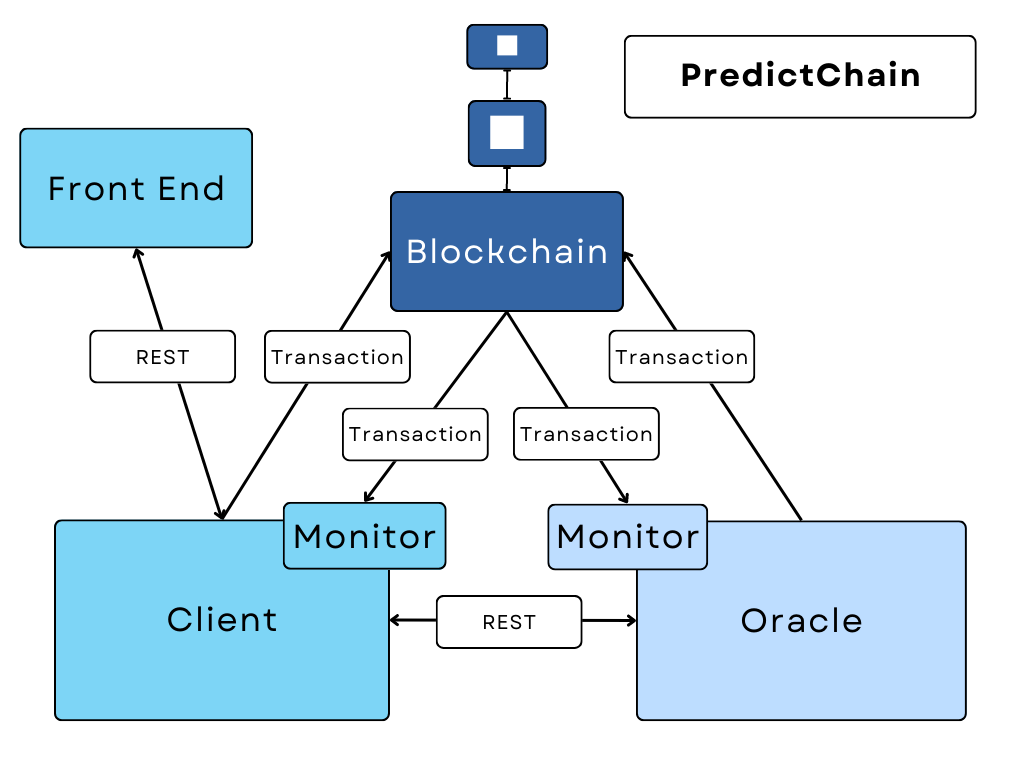
\includegraphics[width=\linewidth]{../../img/detailedDiagram}
            \caption{The architecture of PredictChain}\label{Fig:detailedDiagram}
        \end{minipage}\hfill
        \end{center}
    \end{figure}

    The above diagram illustrates the core components of the system, along with their methods of communication.

    \subsection{The Front End UI}
    Although not directly related to the AI or the blockchain parts of the product, it is still important to discuss the
    UI aspect of our project. The UI sets the user's impression of PredictChain by having multiple pages that create a more
    pleasant experience for the user. For example, the home page talks about our mission, how we differ from our
    competitors and example model sets we provide. The addition of FAQ pages and Meet the Team pages allow users to
    understand who created PredictChain, as well as get answers about any privacy/security concerns they might have.
    Lastly, users can create an account or login to a pre-existing account. Then users are able to use PredictChain
    to its fullest functionality such as adding datasets, checking prices, or querying models with provided datasets.
    The UI talks to the client through a series of REST requests in order to convey this data, later receiving the
    result of the user's actions later through the same means.

    \subsection{The Client}

    The client serves as a middleman between the front end user interface and the blockchain.  It is run as a server,
    serving UI content to the user, taking in requests from the UI, and parsing those requests into a form suitable for
    both the blockchain and for the oracle.  Additionally, the client constantly polls for updates coming from the oracle,
    through the blockchain through its monitor.  These updates are queued and sent to the front end upon request. This
    allows the user to both interact with the blockchain and to see the important updates that come from it.

    \subsection{The Oracle}

    The oracle accomplishes the majority of the other tasks that this project requires.  It constantly polls for updates
    coming from the client, through the blockchain by using its own monitor.  Upon receiving these updates, it begins
    the execution of one of its three main operations.  These are:

    \begin{itemize}
        \item Downloading a user-specified dataset and saving it
        \item Training one of the raw models based on user inputted parameters
        \item Querying one of the trained models on user inputted data and comparing it to the real-world result
    \end{itemize}

    After each of these operations, the oracle sends out several transactions.  These can be either rewards to contributors
    of a model or confirmations/results of the operation that has been performed.

    When working with user-submitted datasets, the oracle uses a handler to manage the operations performed on that dataset.
    The handler can save datasets to a specified environment, load datasets from a specified environment, parse that dataset
    as a pandas dataframe, and split the dataset by the values of one of its attributes.  The environments that the handler's
    recognize are \textit{local} and \textit{IPFS}.  When using either of these environments, the handler abstracts away the
    complexities of working with either of them into a unified interface.

    When working with user-trained models, the oracle uses a similar, common interface.  This interface can create the model
    architecture, train the model on a selected dataset, query the trained model, evaluate its performance, save the model,
    and load it back from a specified environment.  When creating and training a model, the interface chooses among a group
    of archetype or template models.  These models can be a:

    \begin{itemize}
        \item Multi-layered perceptron neural network
        \item Recurrent neural network
        \item Long short-term memory neural networks
        \item Gated recurrent unit neural networks
    \end{itemize}

    Each of these models has a \textit{model\_complexity} attribute.  This is a simple float value, designed to give users
    a general idea of how performant a model can be once trained and serves as a method of calculating the cost of using
    or training that given model.  The attribute itself is calculated using the size of the network and a linear multiplier to
    account for more complex model architectures.  For models like GRUs or LSTMs, the complexity is higher as they are mode complex, and often
    better performing models.  For models like MLPs, the complexity is lower.  This gives the desired effect of faster, simpler
    models being cheaper than the slower, more complex models without any heavy calculations.   The interface abstracts most
    of the complexities of training, querying, and evaluating these models.  The only difference between them is the inclusion
    of several optional parameters.

    \subsection{The Blockchain}

    In PredictChain, the blockchain serves as both a records keeper and a messenger between the client and the oracle.
    This is accomplished by using transactions as a form of direct communication.  With every transaction sent, there is a note.
    This note is a json-encoded string (encoded in base64) that communicates information about the operation that the transaction
    is requesting and arguments for that operation.  The operations in the note are represented by a series
    of op codes.  These codes are abbreviations of the operation name enclosed in angle brackets, for example \textit{<QUERY\_MODEL>}.
    The arguments to these operations are represented as a named dictionary, with each key being the name of the argument and each
    value being the argument itself.  This named strategy allows the program to be very flexible without worrying about the exact
    ordering of the arguments.  Blockchain is quite useful in its role due to its immutability and its transparency.  Using
    a blockchain means that all requests are permanently stored and public, so other users can see what type of models are useful
    for specific datasets and what results those models have produced.

    \subsection{Software and Libraries}

    This project is primarily built in Python, using the Algorand SDK.  The SDK makes interacting with the blockchain
    very straightforward.  Through the tools provided by this library, we can easily read and write transactions from
    the Algorand blockchain.

    Through Python, we also used data science and machine learning libraries such as Pandas
    and Torch.  These libraries encapsulate many of the complexities of data preparation and model training for us.
    By using these libraries, we were able to concentrate on the higher-level functions of the project instead of worrying
    about the lower-level implementation.

    Flask as also an important part of the project.  We used Flask to allow both
    the client and oracle nodes to function as servers.  The client would take in requests from the user and send out
    requests to the oracle.  The oracle would then take in those requests and issue responses.  We chose to use Flask in
    client-oracle communication to cut down on the amount of trivial transactions that would otherwise be made.  For example,
    it would not benefit the accessibility or transparency of the project greatly if the exchanged transactions were
    dominated by simple '\textit{what is the price of \ldots}' requests.

    Additionally, the front end utilizes the React framework and firebase.  React was useful to us as it streamlined the process of making
    dynamic, modular code for the web interface.  Firebase was invaluable for handling administrative tasks such as keeping
    track of registered users and their associated metadata.

    For the recommended configuration of the project, we use Reds as well.  Redis helps to provide a reliable store for
    our metadata about models and datasets in a simple, persistent manner.

    \section{Evaluation}

    % How do you know your solution works? What tests have you performed, and what results have you obtained?
    % If you have acquired any users to try out your system, summarize their reactions and feedback

    While the most definitive evaluation would be to deploy our project and get feedback from actual users, we are limited
    in our time and in our scope.  In place of this, we have devised several tests that are designed to evaluate each
    component of the project on its own and how the entire project functions as a whole.

    \subsection{Transactions}

    The usage of transactions is central to the communications protocol of PredictChain, so making sure the protocol
    functions correctly is critical to the evaluation of the project.  There are few issues with encoding the
    notes and actually sending the transactions, thanks to the SDK.  Where problems can potentially arise is within the
    client and oracle monitors.

    The monitors are classes inside the client and oracle that listen for any transactions that have their node address
    as the recipient.  This listening is done using the Algorand indexer class and a constant polling for new transactions.
    We noticed that this monitor would sometimes skip or duplicate incoming transactions.  As we developed fixes for
    these issues, we constantly evaluated the performance of the monitor.  This was done through programmatically sending
    one or more transactions to the client or oracle address and checking to see how the monitor handled them.  By comparing
    the unique transaction ids of the sent transactions to those processed, we were able to evaluate the monitor,
    identify issues, and create fixes.

    For example, we now constantly update the minimum timestamp the indexer can look for transactions after and we also
    keep a registry of the ids of all past transactions.  This helps to eliminate duplicate transactions getting through.

    \subsection{Models}

    Another critical component of PredictChain is its usage of a variety of models.  At present, all of these models
    are different types of neural networks.  However, these networks are not created equally, with each having different
    qualities, architectures, and outputs.  In order to evaluate the performance of these models, we ran several experiments
    on the models where their hyper-parameters and architectures were kept constant as they were tested.  For this
    evaluation, we measured their performance on our sample dataset, The University of California, Irvine's \textit{Dow Jones
    Index} data set~\cite{dowJones}.  This dataset has 16 different parameters, detailing the attributes of a range of
    stocks from the first half of 2011.  For our usage, we do not eliminate any of these during training, although this
    may be an opportunity for future improvement.  As for the models, they were all initialized with the following parameters:

    \begin{table}[H]
        \begin{center}
            \caption{{Model Evaluation Parameters}}
            \label{tab:evalParams}
            \bgroup
            \def\arraystretch{1.2}
            \begin{tabular}{|c|c|c|}
                \hline\\
                \textbf{Parameter Name} & \textbf{Value} & \textbf{Description}\\
                \hline
                \textit{epochs} & 70 & The number of epochs that the model would train for\\
                \hline
                \textit{target\_attrib} & \textit{close} & \makecell{The attribute that the model was trying to predict,\\this is the daily closing price of the stock}\\
                \hline
                \textit{hidden\_dim} & 5 & The number of neurons in each hidden layer\\
                \hline
                \textit{num\_hidden\_layers} & 1 & The number of hidden layers\\
                \hline
                \textit{time\_lag} & 0 & The number of time steps that pass between the input window and the prediction\\
                \hline
                \textit{training\_lookback} & 10 & The number of time steps that recurrent models receive as input\\
                \hline
                \textit{sub\_split\_value} & 0 & The integer id of the stock to predict, in this case its is \textit{AA} (Alcoa Corp)\\
                \hline
            \end{tabular}
            \egroup
        \end{center}
    \end{table}

    We performed this test on all of our basic model structures, specifically our GRU, LSTM, RNN, and MLP models.
    In the following figures, we show the input data and predictions for each model.  We also show the final loss
    and the final accuracy.  The loss is calculated using the mean absolute error function
    $mae(x, y) = (\Sigma^n_{i=1} |y_i - x_i|) / n$ and our accuracy is calculated using
    $acc(x, y) = \sigma(-mae(x, y)+e^2)$ where $\sigma$ is the sigmoid function.  Our accuracy function is modified
    in this way so that very large losses are registered as somewhat accurate and lower losses are registered as
    very accurate.  This helps to account for the very large losses generated by some of the less performant models.

    The results of our evaluations are as follows:

    \begin{figure}[H]
        \begin{minipage}{0.49\textwidth}
            \centering
            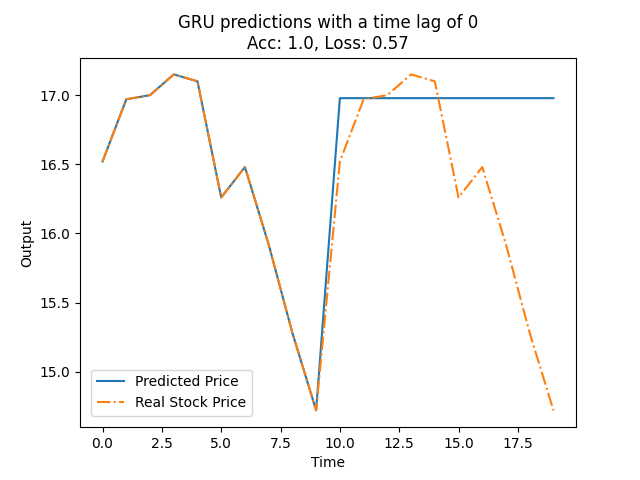
\includegraphics[width=\linewidth]{../../img/gruEval}
            \caption{The results from our GRU model}\label{Fig:gruEval}
        \end{minipage}\hfill
        \begin{minipage}{0.49\textwidth}
            \centering
            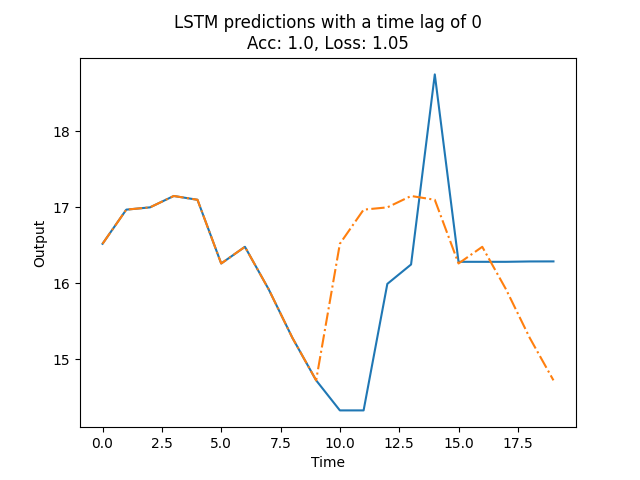
\includegraphics[width=\linewidth]{../../img/lstmEval}
            \caption{The results from our LSTM model}\label{Fig:lstmEval}
        \end{minipage}
    \end{figure}

    \begin{figure}[H]
        \begin{minipage}{0.49\textwidth}
            \centering
            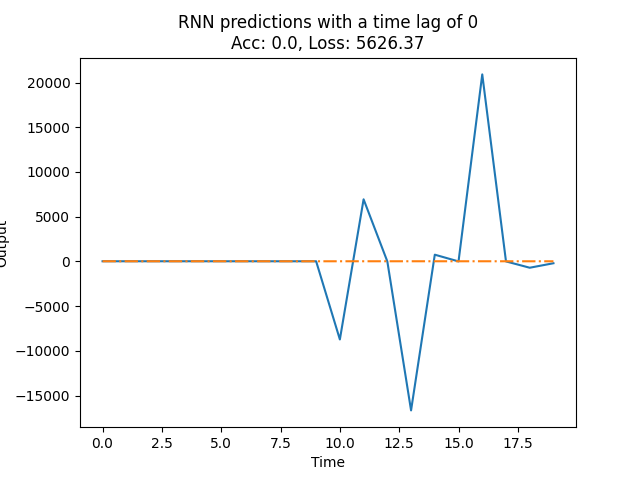
\includegraphics[width=\linewidth]{../../img/rnnEval}
            \caption{The results from our RNN model}\label{Fig:rnnEval}
        \end{minipage}\hfill
        \begin{minipage}{0.49\textwidth}
            \centering
            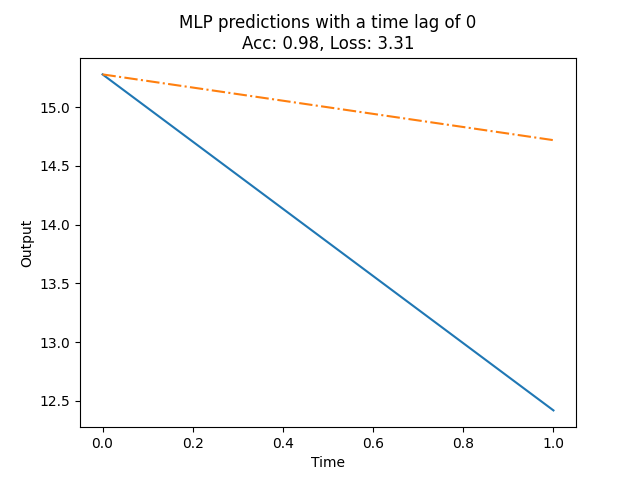
\includegraphics[width=\linewidth]{../../img/mlpEval}
            \caption{The results from our MLP model}\label{Fig:mlpEval}
        \end{minipage}
    \end{figure}

    Each of these results reflects the individual strengths and weaknesses of each model.  As is reflected in our
    \textit{model\_complexity} calculations, the GRU model is the most performant, with a loss of only 0.57.  This is
    closely followed by the LSTM model, which still offers a good prediction, but is slightly less consistent overall.
    In our evaluation of our RNNs, we noticed a good example of the exploding gradients problem.  Without the limits
    provided by the GRU and LSTM models, the predictions of the RNN become increasingly erratic.  Finally, our
    MLP model does not suffer from an exploding gradient, but it does lack the recurrence of the other three models,
    only being able to output one day at a time.

    \subsection{End-To-End Testing}

    \ldots

    \section{Conclusion}

    \subsection{Summary}
    % A short summary of the project

    PredictChain is a blockchain-based marketplace for predictive AI models.
    Through PredictChain, users are able to upload datasets for training predictive models, request that basic models
    be trained on any previously uploaded datasets, or submit queries to those trained models.
    These various models will be operated by a central node or nodes with computing resources available. A variety of
    models will be made available, ranging from cheap, fast, and simple to more expensive, slower, and more powerful.
    This will allow for a large variety of predictive abilities for both simple and complex patterns.  All the past predictions
    form these models will be stored on the blockchain for public viewing.

    \subsection{Limitations}
    % Limitations of the work

    A notable limitation that we experienced during this project was constraints on both our time and the amount of
    hours we could each put into the project.  If this project was worked on for several months longer, the final product
    would be significantly more fleshed out with more features.  If this were more akin to a multi-semester project,
    we would have had the opportunity to add more starting datasets and add a more diverse set of models.

    Another limitation that we had experienced was that we each had other commitments to other classes or activities.
    This limited the amount of hours per week we could each work on improving the project.  To compensate for this, we
    worked together to dynamically adjust our efforts by picking up the work of anyone that was unable to put as much
    time into the project. This strategy helped us to stay on track while maintaining our prior commitments.

    Despite, or perhaps aided by, these limitations, were able to budget our time and distribute the work in such a way
    that out final project is in a functioning state that fulfils our initial objective: to create a prototype for a
    accessible and transparent marketplace for machine learning training and predictions.

    \subsection{Future Work}
    % Potential future work

    As mentioned above, we have several opportunities for improvement that could be accomplished with future work
    into this project.  One major improvement that we could make to the project is the overhaul of the architecture of
    the project.  As mentioned previously, we had briefly considered using many model training nodes instead of a
    centralized node.  Adding this to the project would make the project more decentralized and open up another opportunity
    for community contribution.  This would likely come in the form of users hosting training nodes and being rewarded for
    the quality of models that it produces.  Another potential improvement that could be introduced with future work is
    the addition of a greater variety of models or more example datasets.  Currently we only use neural networks to
    use for predictions.  In future work, we would like to add a more diverse set of models, such as decision trees or
    more statistical models based off of Bayesian inference.

    \pagebreak
    \bibliographystyle{abbrv}
    \bibliography{references}

\end{document}